%% -*- TeX-master: t -*-

\documentclass[draft]{acm_proc_article-sp}

\newcommand{\thetitle}[0]{Propositional Combination of CBI Predicates}

\pagenumbering{arabic}

%%%%%%%%%%%%%%%%%%%%%%%%%%%%%%%%%%%%%%%%%%%%%%%%%%%%%%%%%%%%%%%%%%%%%%%%
%%
%% standard texmf packages
%%

\usepackage{booktabs}
\usepackage{flushend}
\usepackage[final]{graphicx}
\usepackage[dvips]{thumbpdf}

% font selection
\usepackage[T1]{fontenc}
\usepackage{courier}
\usepackage[scaled]{helvet}
\usepackage{mathptmx}

\usepackage[
bookmarks,
breaklinks,
draft=false,
pdftitle={\thetitle},
pdfauthor={Piramanayagam Arumuga Nainar, Ting Chen, Jake Rosin, and Ben Liblit},
% pdfsubject={D.2.4 [Software Engineering]: Software/Program Verification -- statistical methods; D.2.5 [Software Engineering]: Testing and Debugging -- debugging aids, distributed debugging, monitors, tracing; I.5.2 [Pattern Recognition]: Design Methodology -- feature evaluation and selection},
% pdfkeywords={bug isolation, random sampling, invariants, feature selection, statistical debugging},
]{hyperref}

%% \VerbatimFootnotes

%%%%%%%%%%%%%%%%%%%%%%%%%%%%%%%%%%%%%%%%%%%%%%%%%%%%%%%%%%%%%%%%%%%%%%%%
%%
%% unique to this report
%%

\newdef{defn}{Definition}
\newcommand{\defnautorefname}[0]{Definition}

%%%%%%%%%%%%%%%%%%%%%%%%%%%%%%%%%%%%%%%%%%%%%%%%%%%%%%%%%%%%%%%%%%%%%%%%
%%
%% front matter
%%

\title{\thetitle}

\newcommand{\mailto}[1]{\href{mailto:#1@cs.wisc.edu}{#1}}

\numberofauthors{1}
\author{\alignauthor
  Piramanayagam Arumuga Nainar \qquad Ting Chen \qquad Jake Rosin \qquad Ben Liblit \\
  \affaddr{Computer Sciences Department} \\
  \affaddr{University of Wisconsin--Madison} \\
  \email{\{\mailto{arumuga},\mailto{tchen},\mailto{rosin},\mailto{liblit}\}@cs.wisc.edu}}

%%%%%%%%%%%%%%%%%%%%%%%%%%%%%%%%%%%%%%%%%%%%%%%%%%%%%%%%%%%%%%%%%%%%%%%%
%%
%%  document body
%%


\begin{document}

\maketitle

\begin{abstract}
Cooperative Bug Isolation (CBI) is a technique to find bugs in programs that analyzes data collected from program executions.  At each program point, CBI identifies boolean expressions, called as predicates, to be instrumented.  We augment CBI's bug predictive ability by combining these predicates using logical operators (conjunction and disjunction).  The motivation is that a complex predicate will provide more information to the programmer by narrowing down possible program states.  Our experimental results show that the scores of complex predicates are usually higher or atleast comparable to single predicates.  This makes them good indicators of bugs.  We discuss a new metric that uses program structure to quantify the usefulness of complex predicates.  Using this metric, we could eliminate a large number of spurious predicates from consideration.  Finally we discuss the effect of sparse random sampling on the usefulness of complex predicates.

\end{abstract}
% -*- TeX-master: "report" -*-

\section{Introduction}

The Cooperative Bug Isolation (CBI) Project \cite{Liblit:2004:CBI} finds bugs in programs by analyzing reports collected from software executing in the hands of end users.  To use CBI, the software must be compiled with an instrumenting compiler that inserts snippets that evaluate Boolean expressions (called predicates) at various program points.  Predicates are designed to capture program behaviors such as results of function calls, directions of branches or values of variables.  At the end of each execution, the instrumented program generates a report that contains the number of times each predicate was measured, and the number of times each was found to be true.  Statistical debugging is used to analyze these reports and find predicates that are predictive of failure \cite{Liblit:2005:SSBI,Zheng:2006:SDSIMB}.  These predicates are then ranked and presented to the developer.

CBI gathers execution reports by using valuable CPU cycles at end user machines.  It is essential to make those cycles worthwhile by extracting every bit of useful information from them.  However, current statistical analysis algorithms consider predicates in isolation from one another \cite{Liblit:2005:SSBI,Zheng:2006:SDSIMB}.  They overlook potentially useful relations between predicates.  Predicates are expressions involving program variables at different program points and hence may be related by control and data dependences.  We propose to capture these relations by building \emph{complex predicates} from the set of currently instrumented predicates (which we refer to as \emph{simple predicates}).  Since predicates are Boolean expressions, they are combined using logical operators (such as conjunction and disjunction).  We construct complex predicates and include them in the input to the statistical analysis algorithms.

There are two approaches to combine predicates using logical operators:
\begin{enumerate}
\item Explicitly monitor the complex predicate by changing the output of the instrumenting compiler.
\item Estimate the value of the complex predicate from the values of its components.
\end{enumerate}

The first approach will yield a precise value but needs significant modifications to existing infrastructure.  The second approach will be less precise (as described later) but requires only few modifications to existing infrastructure (and none to the instrumenting compiler).  In this project, we implement the second approach, that will serve as a proof of concept for complex predicates, as well as a justification for a future attempt at incorporating them into the compiler.

The remainder of this report is organized as follows.  \autoref{sec-bground} introduces CBI and explains the motivation for complex predicates.  \autoref{sec-complex-preds} gives a precise definition of complex predicates and discusses the trade-offs in our implementation.  \autoref{sec-metrics} describes two metrics to evaluate the usefulness of a complex predicate.  \autoref{sec-qual} describes two case studies that demonstrate the usefulness of complex predicates.  

\autoref{sec-quant} presents the results of experiments conducted on a large suite of test programs.  \autoref{sec-sampling} discusses the effect of sparse random sampling on complex predicates.  Sparse random sampling is a technique used by CBI to reduce the runtime overhead on the instrumented programs.  \autoref{sec-rw} discusses work related to CBI in the context of complex predicate generation.  \autoref{sec-conc} concludes.

% -*- TeX-master: "report" -*-

\newcommand{\rhythmbox}{\textsc{Rhythmbox}\xspace}
% Copied from Ben's PLDI-2004 paper.  --Jake

\section{Background}
\label{sec-bground}
CBI uses lightweight instrumentation to collect feedback reports that contain truth values of predicates in an execution as well as the outcome (e.g., crash or non-crash) of the execution.  A large number of these reports are collected and analyzed using statistical debugging techniques.  Liblit et al. \cite{Liblit:2005:SSBI} compute a numeric $\Importance$ score corresponding to each predicate, define as follows.

The truth values of a predicate $p$ from all the runs can be aggregated into four values:

\begin{enumerate}
\item $\obs{S}{p}$ and $\obs{F}{p}$, the number of successful and failed runs respectively, in which the value of $p$ was evaluated.
\item $S(p)$ and $F(p)$, the number of successful and failed runs respectively, in which the value of $p$ was evaluated and was found to be true.
\end{enumerate}

Using these values, two scores of bug relevance are calculated.  They are:
\begin{enumerate}
\item $F(p)$.  A good predictor must predict a large number of failed runs.
\item $\Increase(p)$, the amount by which $p$ being true increases the probability of failure over simply reaching the line where p is defined.  It is computed as follows:
\end{enumerate}

\begin{equation}
\label{eqn1}
\Increase(p) \equiv
\frac{F(p)}{S(p) + F(p)}
-
\frac{\obs{F}{p}}{\obs{S}{p} + \obs{F}{p}}
\end{equation}

Both of these scores are independent but good dimensions of a bug predictor.  These dimensions are combined into a single value by taking their harmonic mean.  Since $\Increase(p)$ is bounded by 1, the $F(p)$ component in $\Importance$ is normalized over the total number of failed runs $\NumF$ after a logarithmic transformation.  The overall metric is:
\begin{equation}
\label{eqn2}
\Importance(p) \equiv
\frac{2}{%
  \frac{1}{\Increase(p)}
  +
  \frac{1}{log(F(p)) / log(\NumF)}}
\end{equation}

To eliminate different predicates that predict the same bug, only the top ranked predictor is presented to the user.  To handle the case where multiple bugs are present, all the failed runs in which the top predicate is true are eliminated and the remaining predicates are ranked by recomputing their scores in the remaining set of runs.  This process of eliminating runs continues until there are no remaining failed runs or no remaining predicates.

The output of the analysis will contain the list of predicates that had the highest score during any iteration of the redundancy elimination algorithm.  This list may be used by a programmer to identify areas of the program related to faulty behavior.  Liblit et al. discovered previously unknown bugs in \texttt{bc} \cite{Liblit:2003:BIRPS}, \texttt{exif} \cite{Liblit:2005:SSBI} and \rhythmbox \cite{Liblit:2005:SSBI} by employing this method.

The list of bug predictors can alternately be used as input to an automated analysis tool, such as \textsc{BTrace} \cite{Lal:2006:POPAD}. \textsc{BTrace} finds the shortest control- and dataflow-feasible path in the program that visits a given set of bug predictors.  This analysis allows a programmer to examine the fault-predicting behavior even if the connection to a bug is not easily identifiable, or if the predictors are numerous or complex enough to overwhelm a programmer examining them directly.

\subsection{Expected Benefits}
A single predicate can be thought of as partitioning the space of all runs into two subspaces: those satisfying the predicate and those not.  The more closely these partitions match the subspaces where the bug is expressed or not, the better the predicate is as a bug predictor.  A \emph{perfect bug predictor} divides the space of runs into these subspaces exactly.  Generally speaking, the closer a predictor is to perfect the more informative it is to a programmer.  If a bug has a simple cause, and this cause corresponds well to a simple predicate, then a simple analysis is sufficient.

A richer language of candidate bug predictors can describe more complex shapes within the set of runs.  This allows predictors for bugs with more complicated causes.  When predicates do not adequately match the complexity of the bugs they predict the results are \emph{super-} and \emph{sub-bug predictors}, an aspect of statistical debugging first identified by Liblit et al. \cite{Liblit:2005:SSBI}.

A \emph{super-bug predictor} is one which correctly partitions all (or most) expressions of the bug, but also predicts the bug in a large number of runs where it did not occur.  In other words, it is not a specific enough predictor of the bug.  In information-retrieval terms, a super-bug predictor has high recall but low precision.  A possible (but not the only) cause for super-bug predictors is a non-deterministic bug that does not necessarily cause a failure when it is triggered.  False positives could be reduced or eliminated by taking a conjunction of this predictor with another predicate that captures another aspect of the bug; the resulting partitioning would more closely match the bug's behavior.

A \emph{sub-bug predictor} is one that correctly partitions some (but not all) expressions of the bug.  In other words, it is not sensitive enough to predict all instances of the bug.  In information-retrieval terms, a sub-bug predictor has high precision but low recall.  False negatives could be reduced or eliminated by taking a disjunction with another predictor which captures other instances of the bug; as before the resulting predicate would serve as a more accurate predictor.  It is important to note that in software with multiple bugs, the analysis may find a disjunction of predictors of individual bugs as a predictor for the whole set of failures.  The user should keep this in mind while using a disjunction predictor to track down a bug.

The bug predictors which result from combining simple predicates can be conjoined or disjoined again, eliminating false positives and false negatives to approach a perfect predictor.  Finding a predicate which perfectly predicts the expression of a complex bug may be infeasible, but statistical bug isolation does not require one, and a complex predicate which predicts a bug more accurately than any simple predicate is useful even if imperfect.

\section{Complex Predicates}
\label{sec-complex-preds}
\section{Usefulness Metrics for Complex Predicates}
\label{sec-metrics}
While complex predicates could help to better predict bugs, in the
worst case, there will be a quadratic increase in the number of
possible combinations of two single predicates. In our
experiments, we often observe hundreds of complex predicates with
similar or even identical high scores. The overwhelming number of
predicates makes it extremely laborious for users to find the true
cause of the problem and then debug. In this section, we propose two metrics
to reduce the number of complex predicates.

The first metric is to model the debugging effort required 
from the programmer as a filtering metric.  We use the metric defined
in ~\cite{1062522} for this purpose.  In this metric, the score of a predicate
as the fraction of code that can be ignored while searching for the bug.
We use a similar metric called $effort$ for a complex predicate.

\begin{defn}
\label{dfn4}
The effort required by a programmer while using a complex predicate 
$C = \phi(p_1, p_2)$ as inversely proportional to the fraction 
of code that can be ignored while searching for $p_1$ from $p_2$ or
vice versa.
\end{defn}

The idea behind this metric is that the larger the distance between
the two predicates, the greater the effort requried.  Also, if a 
large number of other branches seen during the search, the programmer
should keep track of these dependencies too.  Like ~\cite{1062522}, 
we use the program dependence graph (PDG) of to model the program rather
than the source code.

The second metric is to consider the correlation between the two predicates.  Intuitively a complex predicate with two relatively independent predicates is less interesting because it doesn't provide much help to the users in finding anything new, besides the two individual predicates.  The correlation between two predicates is defined based on the program dependency graph.  Given a single predicate $P$, we define its $predecessor\ set$ as the set of vertices in the PDG that can influence the outcome of $P$.

\begin{defn}
\label{dfn5}
The correlation between two predicates of a complex predicate is defined as the number of vertices in the intersection of the two predecessor sets.
\end{defn}

The idea behind this metric is that a larger intersection between the $predecessor\ sets$ means that it is possible that they are closely related.  We use CodeSurfer[] to build the PDG of a program and compute these two metrics.

The above two metrics could be applied both $proactively$ and $reactively$.  A proactive use of the metrics will prune away complex predicates whose metric values fall below a certain threshold of usefulness.  This will eliminate them from being computed and hence a performance optimization.  A reactive use of the metrics will retain all the predicates but break ties by giving higher ranks to those with higher values of the metrics. This is desirable if neither computing time or space is a concern.



\section{Case Studies}
\label{sec-qual}
\section{Experiments}
\label{sec-quant}
\begin{figure}
  \centering
  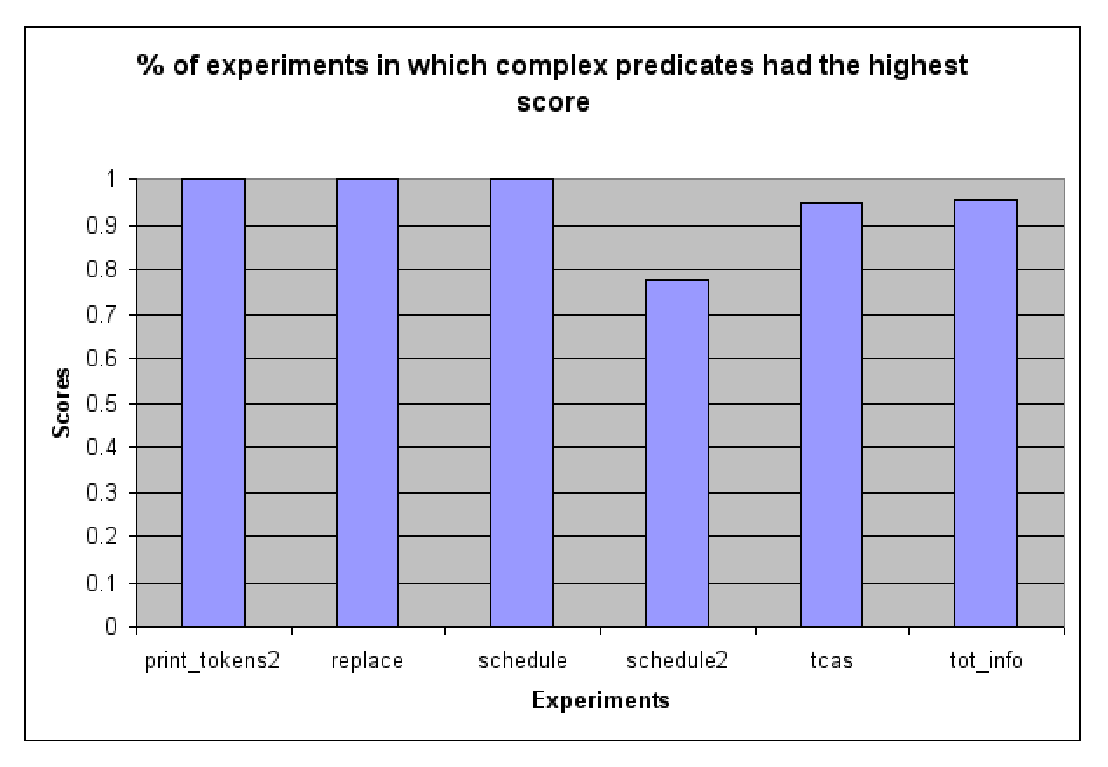
\includegraphics[width=\columnwidth]{charts/top-pred}  
  \caption{Complex predicates having the highest score}
  \label{fig-top-pred}
\end{figure}

\begin{figure}
  \centering
  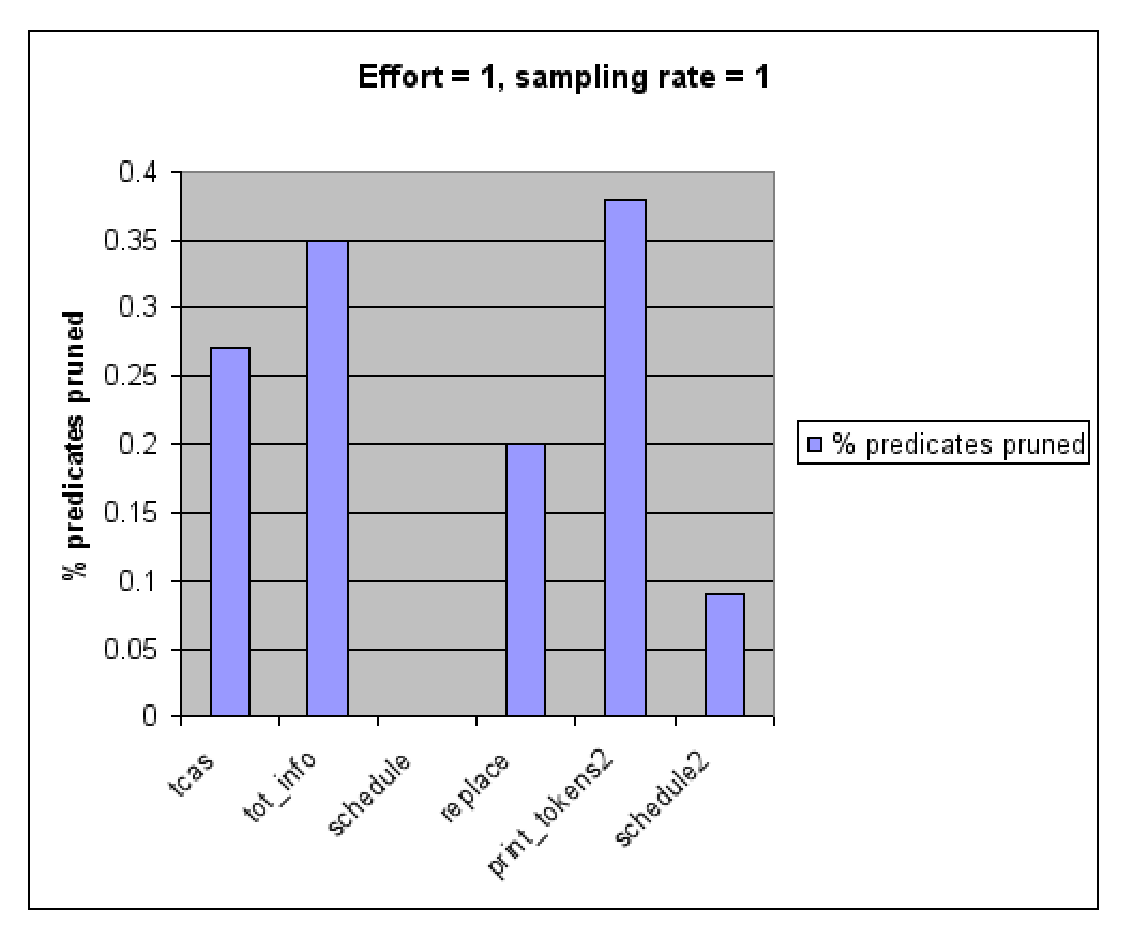
\includegraphics[width=\columnwidth]{charts/pruning}
  \caption{Improvement from pruning}
  \label{fig-pruning}
\end{figure}

\begin{figure}
  \centering
  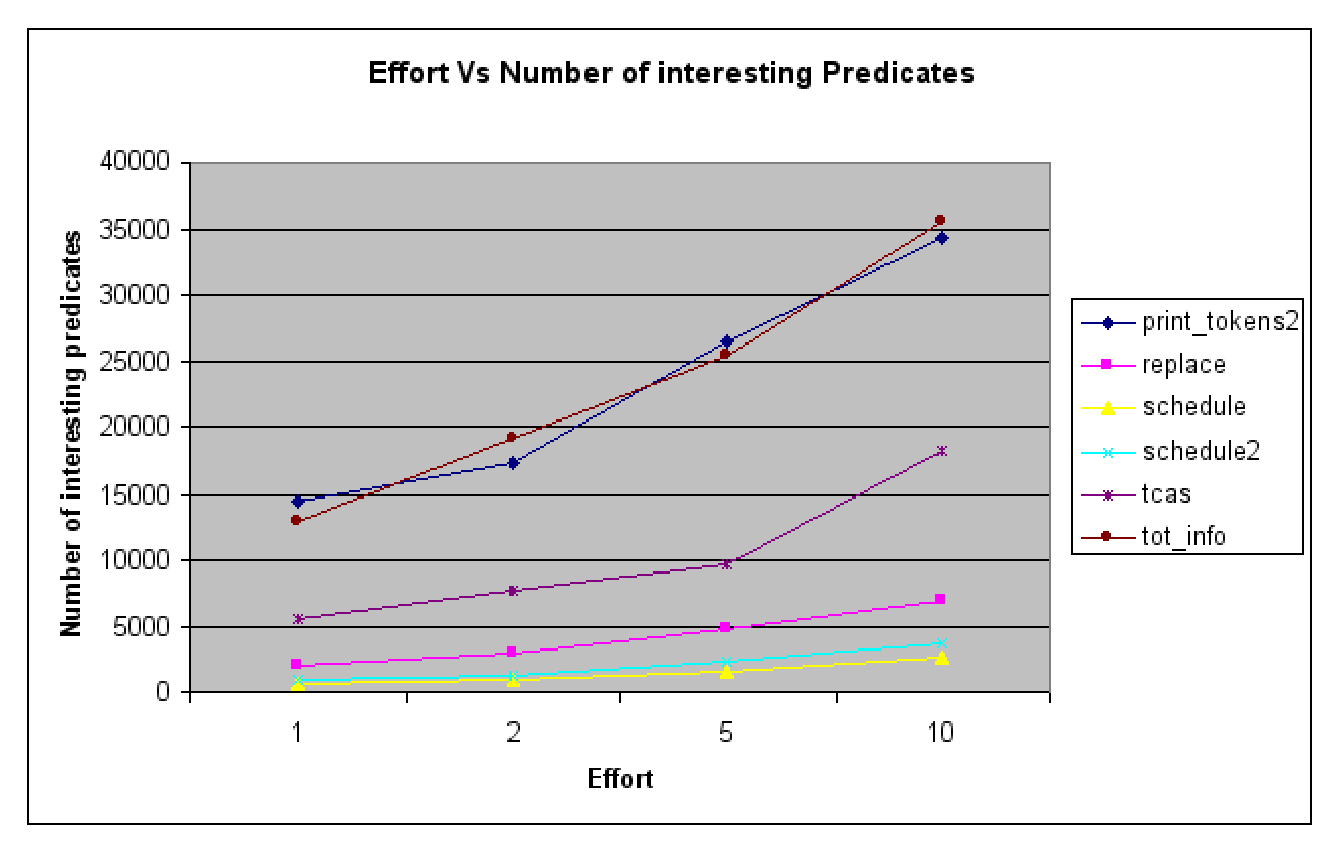
\includegraphics[width=\columnwidth]{charts/effort}
  \caption{Variation of number of interesting predicates with $effort$}
  \label{fig-effort}
\end{figure}

\begin{figure*}
  \centering
  $\begin{array}{cc}
    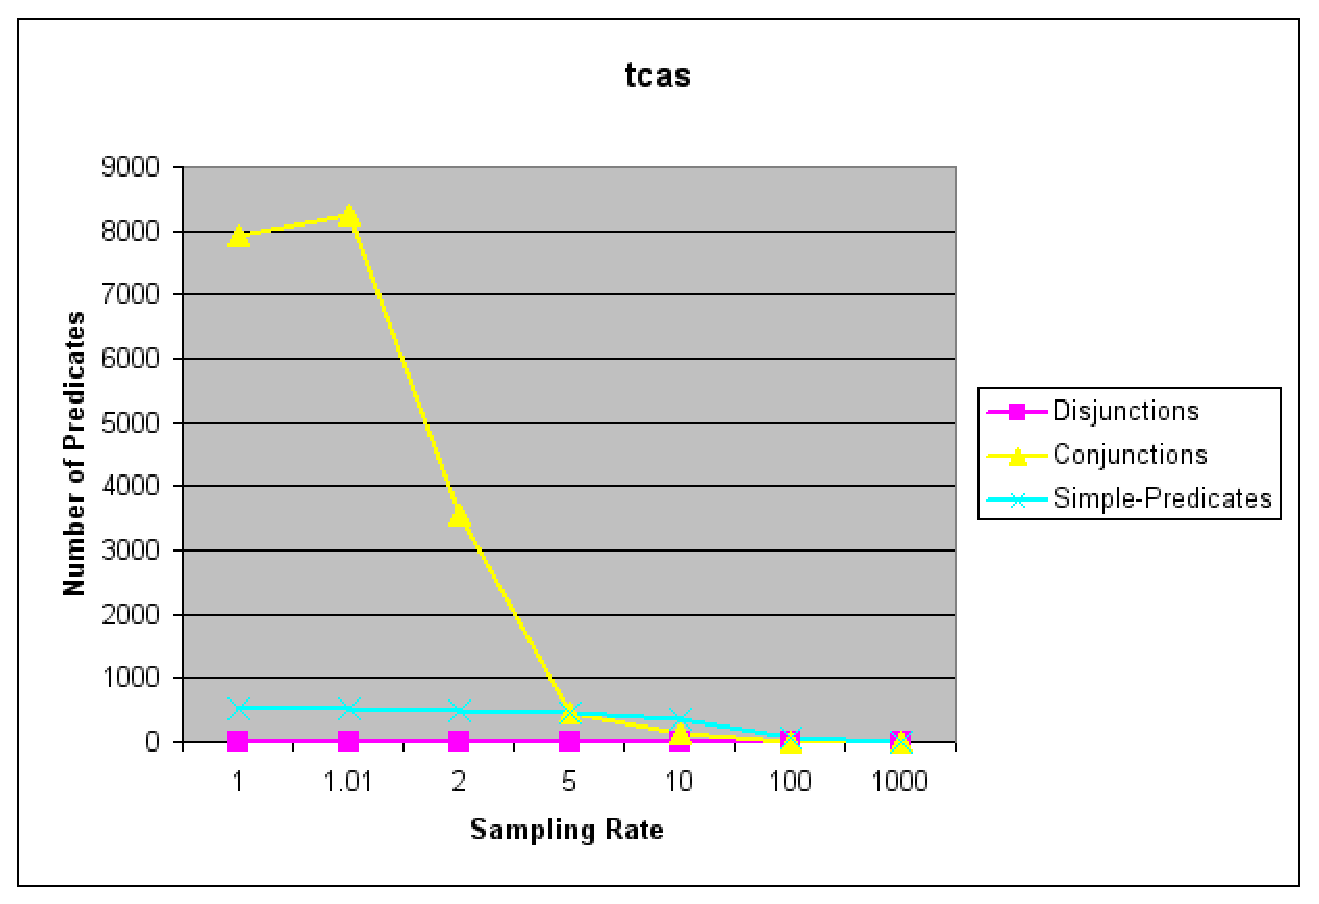
\includegraphics[width=\columnwidth]{charts/tcas} & 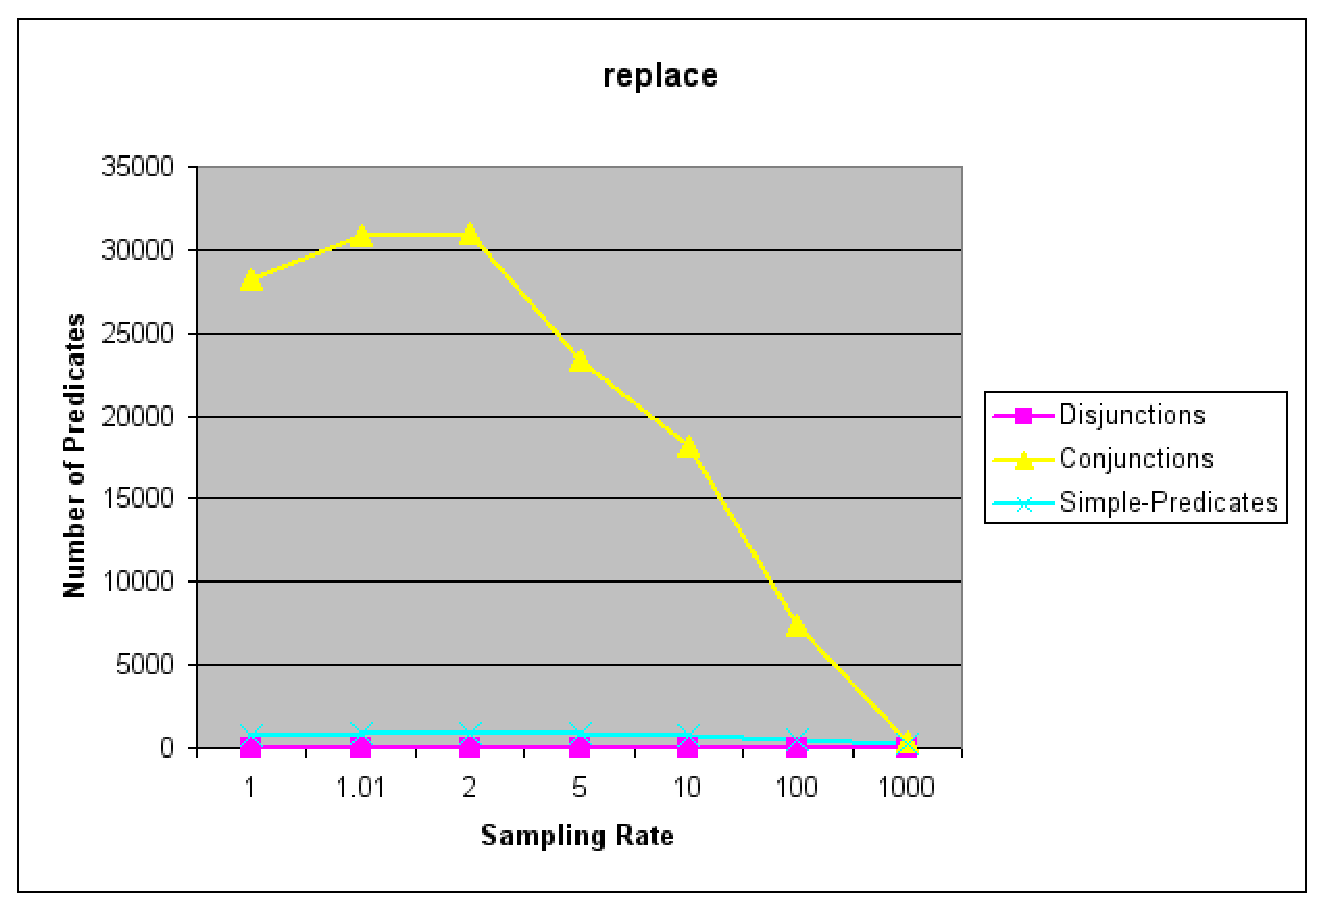
\includegraphics[width=\columnwidth]{charts/replace} \\
    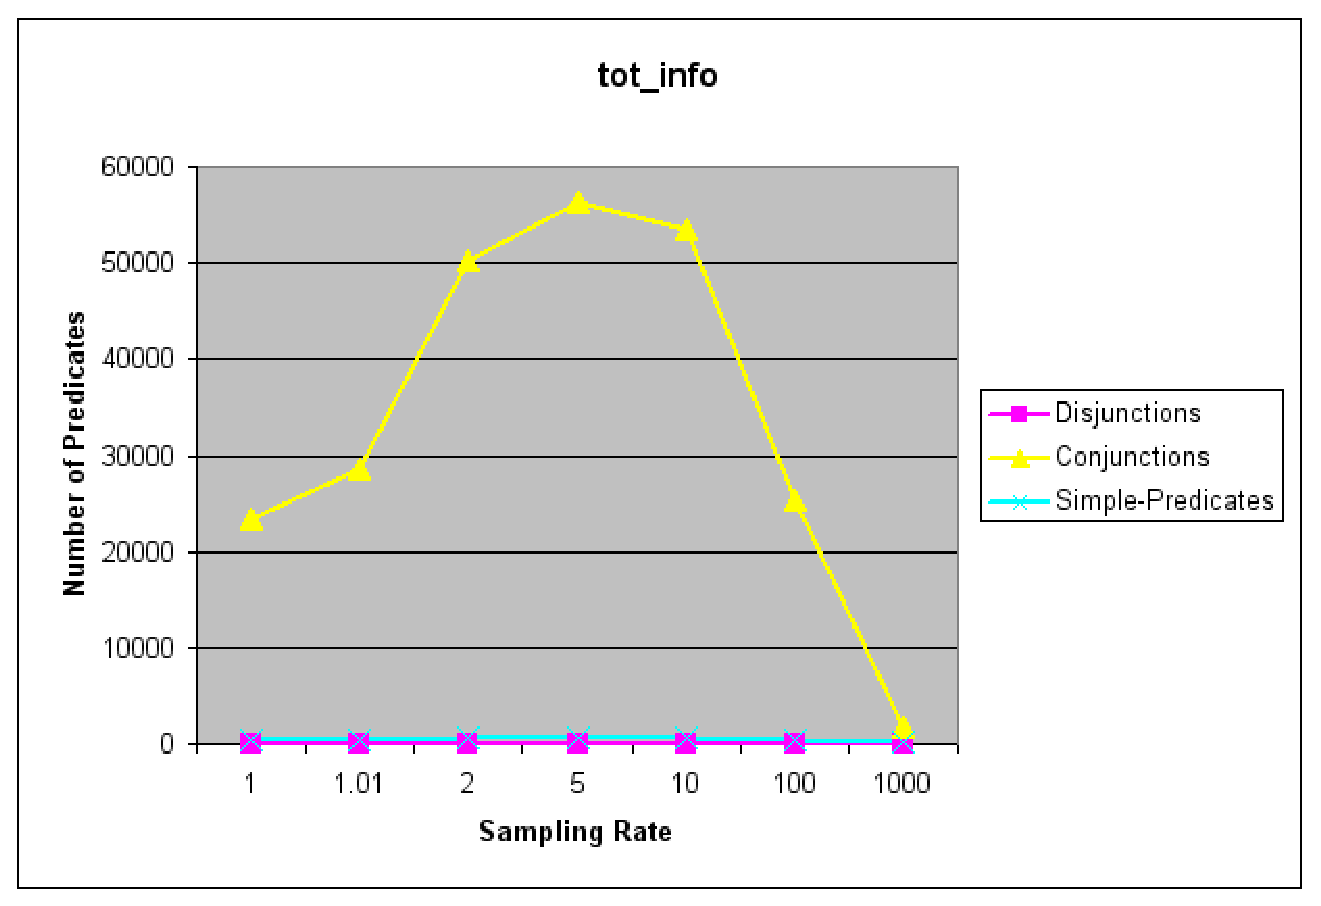
\includegraphics[width=\columnwidth]{charts/tot_info} & 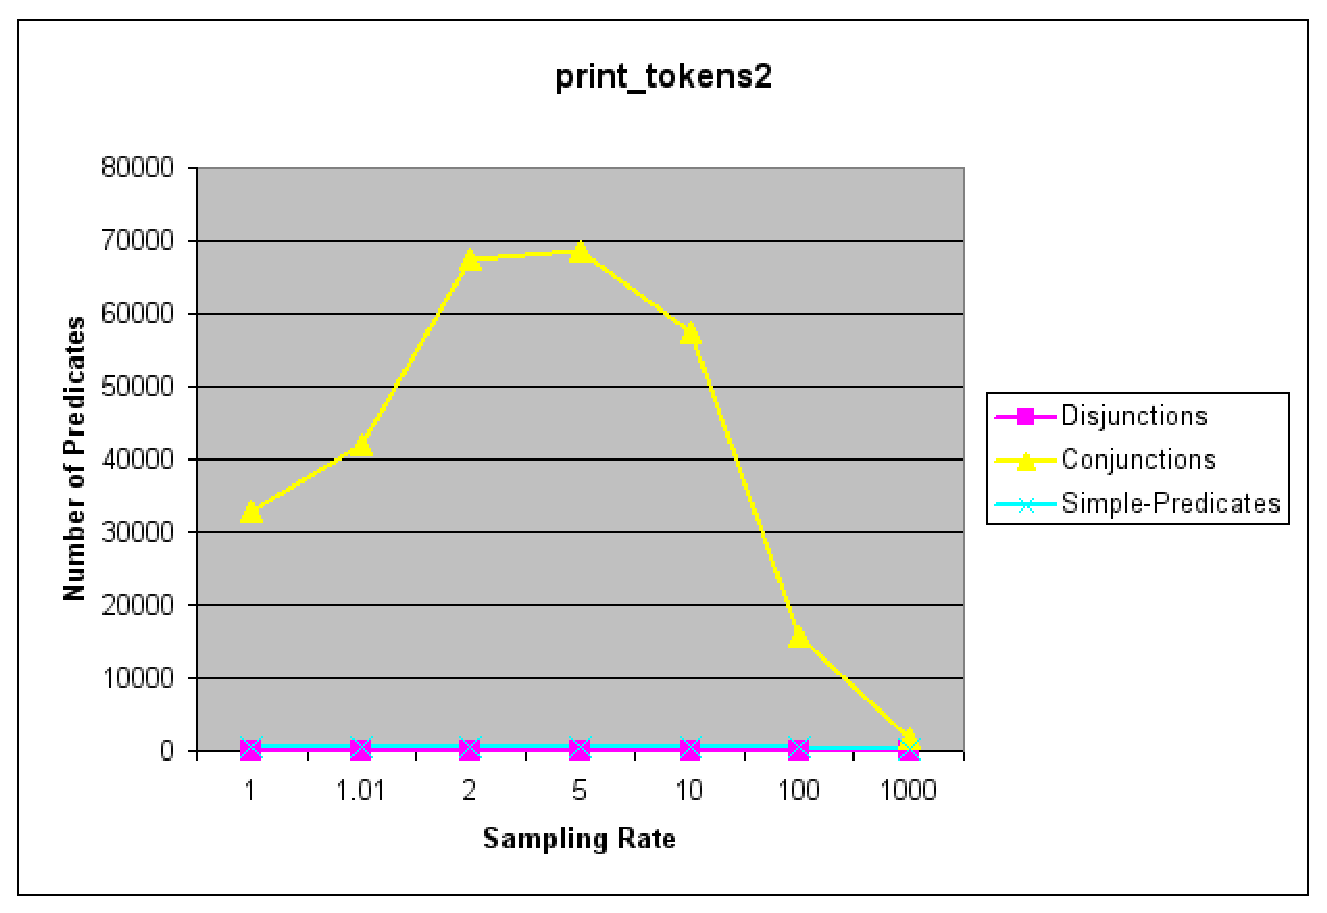
\includegraphics[width=\columnwidth]{charts/print_tokens2} \\
    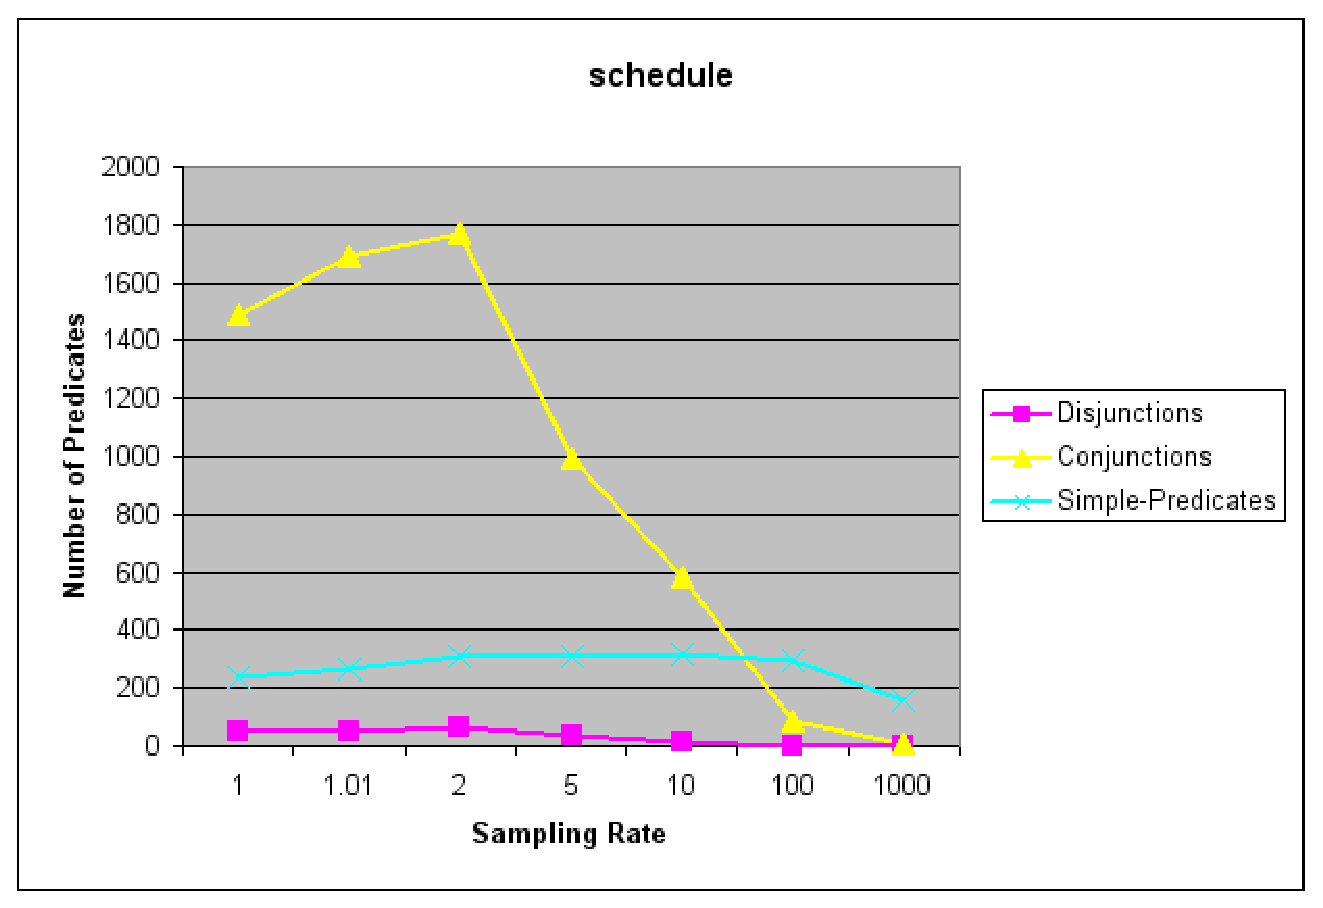
\includegraphics[width=\columnwidth]{charts/schedule} & 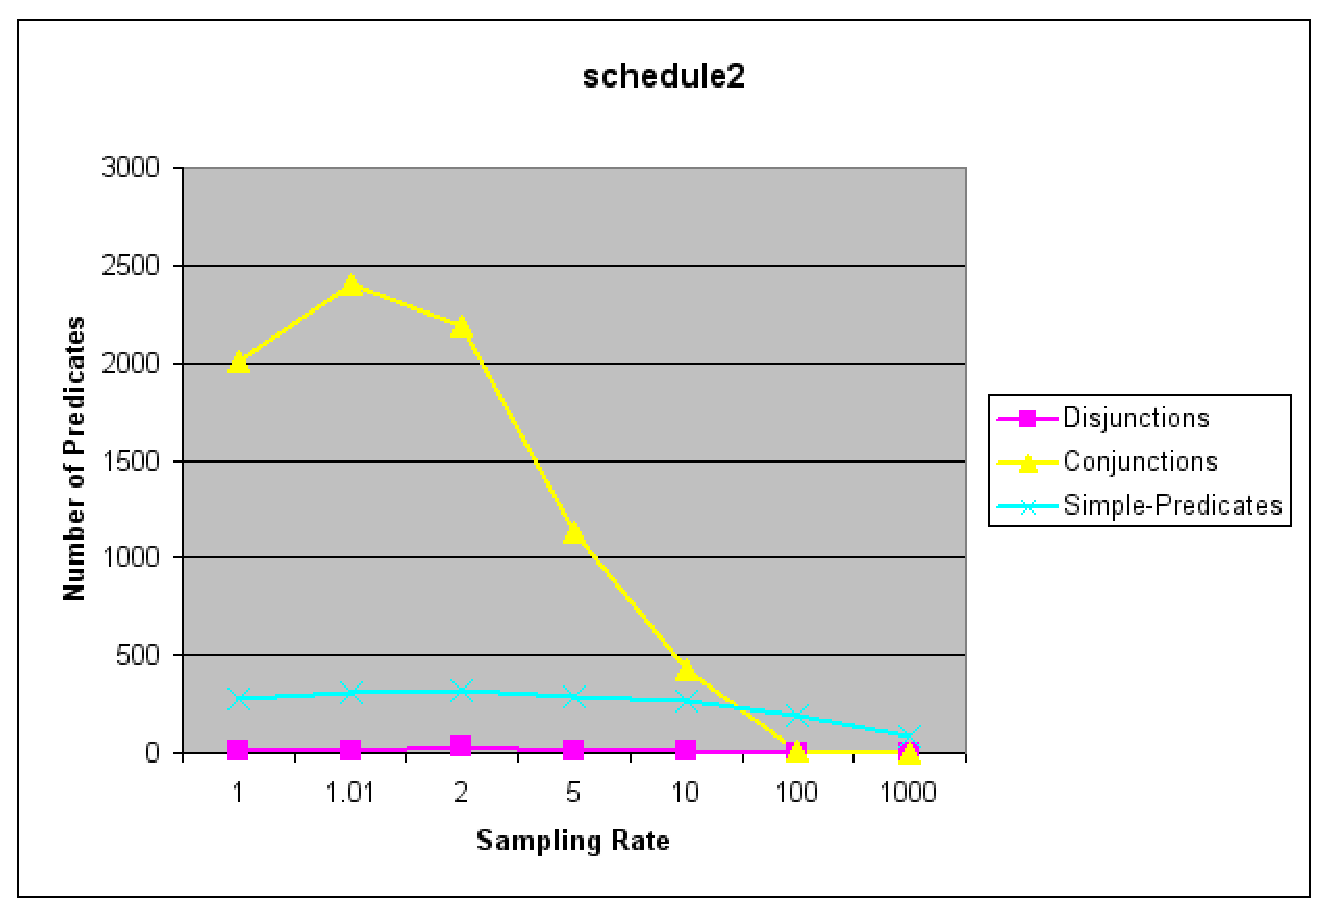
\includegraphics[width=\columnwidth]{charts/schedule2} \\
  \end{array}$
  \caption{Sampling Rate vs. Number of Predicates}
  \label{fig-sampling}
\end{figure*}

This section presents quantitative data about the ideas presented in previous sections.  This data was collected using the Siemens test suite~\cite{257766}.  There are two configurable parameters for the experiments: the rate of sampling and $effort$ (described in ~\autoref{sec-metrics}).  Unless specified, the default sampling rate is 1 (i.e. complete data collection) and the default $effort$ is 5\% (only predicates that are reachable from each other by exploring less than 5\% of the program are considered).

\subsection{Top Scoring Predicates}
~\autoref{fig-top-pred} plots the percentage of variants within each program for which a complex predicate had the highest score among all predicates.  The value is 100\% for \texttt{print\_tokens2, replace} and \texttt{schedule} and is close to 100\% for the other programs.  The results shown in ~\autoref{fig-top-pred} combined with the case studies in ~\autoref{sec-qual} demonstrates the usefulness of complex predicates.

\subsection{Improvement from Pruning}
~\autoref{fig-pruning} shows the percentage of complex predicates that are pruned by the optimizations discussed in ~\autoref{sec-pruning} and the metrics in ~\autoref{sec-metrics}.  For each program, the y-axis shows the contribution of the two kinds of pruning.  On average, the usefulness metrics prune 54\% of complex predicates and the optimizations in ~\autoref{sec-pruning} prune 15\% of complex predicates.  Only 31\% of the complex predicates are actually computed.

\subsection{Effect of the $Effort$ Parameter}
~\autoref{fig-effort} has one curve for each program showing how the number of interesting predicates (~\autoref{dfn3}) varies at four different values - 1, 2, 5, 10 for $effort$.  As expected, as $effort$ increases more predicates are evaluated and so more interesting predicates are found.  This experiment serves as a sanity check for the implementation.

\subsection{Effect of Sampling Rate}
\label{sec-sampling}
The dependence between sampling rate and the number of interesting predicates (both complex and simple) is plotted in ~\autoref{fig-sampling}.  ~\autoref{fig-sampling} has one chart per program with sampling rates in the $x-$axis and the average number of interesting conjunctions, disjunctions and simple predicates in the $y-$axis.  The number of interesting disjunctions is always very low (order of tens) compared to interesting conjunctions.  So the plot for interesting complex predicates closely follows the plot for conjunctions.  At sampling rates higher than 10, there is a sharp drop in the number of interesting conjunctions.  This is because with a sampling rate of $N$, the chance of observing a complex predicate is close $\frac{1}{N^2}$ {\footnote{it is not equal to $\frac{1}{N^2}$ because of short circuiting boolean operations}}.  Despite the sharp drop, the number of interesting conjunctions is still comparable to the number of interesting simple predicates.  This shows that sparse random sampling is not a significant detriment in finding interesting complex predicates.

A puzzling trend in ~\autoref{fig-sampling} is that interesting conjunctions increases for a brief interval before dropping off.  This trend is consistent across all programs.  This can be due to two reasons:
\begin{enumerate}
\item Consider the $Increase$ score (Eqn ~\ref{eqn1}).  Sampling may be reducing the number of $observed$ runs in which a conjunction was true without affecting the $true$ runs.  This could happen because we do not collect sampled data directly but use scripts to down sample a data set collected with no sampling.  Because of binarization of counts, down sampling of a count from 100 to 99 does not affect the score whereas down sampling from 1 to 0 affects the score. 
\item The script that does down sampling uses the standard pseudo random number generator.  Usually for experiments that use such random data, the values are averaged over multiple trials to get a confident estimate of the results.  We weren't able to conduct multiple trials because of time constraints.
\end{enumerate}

% -*- TeX-master: "report" -*-

\section{Related Work}
\label{sec-rw}
Daikon \cite{ErnstPGMPTX2006} detects invariants in a program by observing values computed by it.  It can compute complex invariants by combining program variables and operators like sum, max, etc.\ on collection (e.g., array) objects.  Invariants are predicates that must be true in correct executions.  Dodoo et al. \cite{ErnstDRAFT} extend the work to compute implications of the form $a \implies b$.  Our study is different from this in two ways.  First, the data we have (bit vector of predicate counts) is different from what Daikon uses (values of variables at different points).  So the fundamental techniques in our approach and Dodoo et al. \cite{ErnstDRAFT} are different.  Secondly, our project also aims at processing a sparse random sample of predicate values, whereas Daikon requires complete execution traces.  DIDUCE \cite{581377} is inspired by Daikon and identifies predicates that are true in failed runs.  SOBER \cite{1081753} is a statistical debugging tool similar to CBI\@.  Neither of these approaches tries to construct complex predicates.

\section{Conclusion}
\label{sec-conc}
We have demonstrated that complex predicates are useful predictors of bugs.  Our experiments show qualitative and quantitative evidence that complex predicates can improve the current statistical analysis used by CBI.  We describe two optimizations that make the task of computing complex predicates feasible.  First is a numeric estimate on the upper bound of the score of a complex predicate.  The second is a metric that quantifies the usefulness of a complex predicate.  Even after these, the computational complexity is still high and requires further optimizations.  The metrics described in section ~\ref{sec-metrics} help reduce the number of spurious predicates.  But the metrics are not perfect as good bug predictors are still swamped by less useful ones.  The algorithm described in ~\cite{Zheng:2006:SDSIMB} may solve this problem as it was designed with the goal of handling multiple predictors for the same bug.

\bibliographystyle{abbrv}
\bibliography{local}

\end{document}
